\begin{figure}[t]
\centering
\begin{minipage}[b]{0.45\linewidth}
\centering
\subfloat[][Tadpole]{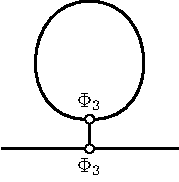
\includegraphics{fig_3_3_feynman_diagram/tadpole.pdf}}
\end{minipage}
\begin{minipage}[b]{0.45\linewidth}
\centering
\subfloat[][Loop]{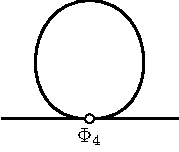
\includegraphics{fig_3_3_feynman_diagram/loop.pdf}}
\end{minipage}

\begin{minipage}[b]{0.45\linewidth}
\centering
\subfloat[][Bubble]{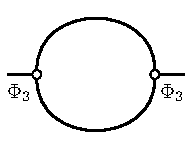
\includegraphics{fig_3_3_feynman_diagram/bubble.pdf}}
\end{minipage}
\begin{minipage}[b]{0.45\linewidth}
\centering
\subfloat[][4ph]{\includegraphics{fig_3_3_feynman_diagram/4ph.pdf}}
\end{minipage}
\caption{Feynman diagrams of phonon self energies. Solid lines and open circles represent phonon propergators and phonon vertexes, respectively.}
\label{fig:diagram}
\end{figure}